\section{A rank-five K3 wall crossing}\label{sec:application}

We construct one bundle-moduli problem to which all the preceding
analytic results apply. It has three distinct stable factors,
multiplicities $(2,2,1)$ and two independent polarization parameters.
The two noncommutative multiplicity groups act on a common extension
space. The three-edge cycle also removes the sign symmetry that would
give the quadratic error automatically.

\subsection{The surface and the polystable bundle}
Consider the lattice with basis $H,a,b$ and Gram matrix
\begin{equation}\label{eq:k3-lattice}
 \begin{pmatrix}2&0&0\\0&-4&2\\0&2&-4\end{pmatrix}.
\end{equation}
In three hyperbolic planes with bases $e_i,f_i$, $e_i\cdot f_i=1$,
the vectors
\[
 H=e_0+f_0,\qquad a=e_1-2f_1,\qquad b=2f_1+e_2-2f_2
\]
have these pairings. Their $e_0,e_1,e_2$ coordinates form an identity
minor, so the embedding is primitive. The lattice is even of signature
$(1,2)$. Morrison's realization theorem
\cite[Corollary~1.9(i)]{Mor84} gives a projective K3 surface with
exactly this N\'eron--Severi lattice.

The class $H$ can be made ample by choosing the marking.
Indeed its orthogonal lattice has square
$-4(p^2+q^2-pq)$ and contains no class of square $-2$.
After choosing the positive-cone component, $H$ lies in the interior
of a root chamber. The root-reflection group carries it to the
ample chamber; compose the marking with this action
\cite[\S1, Theorem~3.1 and Corollary~3.2]{Dol96}.
This does not assert that the full Picard lattice is root-free:
$H+a$ has square $-2$.

Let $L_1,L_2,L_3$ be the line bundles with classes $a,b,-a-b$.
Their squares are $-4$ and their $H$-degrees are zero.
Pairwise differences have square $-12$ and no sections in either
sign: a nonzero effective divisor has positive $H$-degree, and
the line bundles are distinct. Serre duality and Riemann--Roch give
\begin{equation}\label{eq:line-exts}
 \dim\Ext^1(L_i,L_j)=4\quad(i\ne j),\qquad
 \dim\Ext^\bullet(L_i,L_i)=(1,0,1).
\end{equation}
Moreover
$\chi(L_i(nH))=2+\tfrac12(c_1(L_i)+nH)^2=n^2$.
Thus
\[
 E_0=L_1^{\oplus2}\oplus L_2^{\oplus2}\oplus L_3
\]
is both slope and Gieseker polystable at $H$.
Its invariants are
\begin{equation}\label{eq:mukai-example}
 \rank E_0=5,\qquad c_1(E_0)=a+b,\qquad c_2(E_0)=8,\qquad
 v(E_0)=(5,a+b,-5),\qquad v(E_0)^2=46.
\end{equation}
The Mukai vector is primitive. The extension space has complex
dimension $64$, and the effective group
$(GL_2\times GL_2\times GL_1)/\CC^*$ has dimension $8$.

For small real $(t,u)$ the class $H+ta+ub$ is K\"ahler.
Choose its smoothly varying Ricci-flat forms. The real moment
parameter in \eqref{eq:geometric-parameter} is
\begin{equation}\label{eq:two-parameter}
 \zeta(t,u)=\frac{2\pi}{5}(18t-12u,\ -12t+18u,\ -12t-12u).
\end{equation}
Its image is the entire plane $2\zeta_1+2\zeta_2+\zeta_3=0$.
Thus the analytic family realizes every sufficiently small real
central parameter, not just one prescribed ray.

\subsection{Simple zero-level representations}
Orient the edges $12,13,23$ toward the larger index. On each edge
take four forward arrows and four reverse arrows. For rectangular
matrices $C,D$ put
\begin{equation}\label{eq:paired-seed}
 (A_1,A_2,A_3,A_4)=(C,C,D,D),\qquad
 (B_1,B_2,B_3,B_4)=(C^*,-C^*,D^*,-D^*).
\end{equation}
The complex moment cancels between the two copies of each matrix;
each forward/reverse pair cancels in the real moment.
For dimensions $(2,2,1)$ use
\[
 (C_{12},D_{12})=
 \left(I_2,\begin{pmatrix}0&1\\0&0\end{pmatrix}\right),
 \qquad
 (C_{13},D_{13})=(C_{23},D_{23})
 =\bigl((1,0),(0,1)\bigr).
\]

\begin{lemma}\label{lem:example-simple}
These arrows give a module-simple point in the complex and real
zero moment fiber. The same construction gives simple zero-level
representations for every summand in Table~\ref{tab:walls}.
\end{lemma}
\begin{proof}
An endomorphism commutes with $I_2$ on edge $12$, so its first two
vertex matrices agree. That matrix commutes with the displayed
nilpotent and its adjoint, hence is scalar. The coordinate rows
make its scalar agree with the scalar at vertex $3$.
Thus its endomorphism algebra is $\CC$.
The directed arrow collection is closed under adjoints up to sign,
so any subrepresentation has an invariant orthogonal complement.
Its orthogonal projection would be a nonscalar endomorphism if
the subrepresentation were nonzero and proper. This proves
module simplicity, rather than only the Schur property.

For the other vectors, on edges of sizes $(1,2)$ use the two
coordinate columns, on $(2,1)$ the two coordinate rows, and on
$(1,1)$ use $C=1,D=0$. Use the same $(I_2,D)$ at a $(2,2)$
edge when present. These arrows and their adjoints force scalar
endomorphisms at every connected vertex and the scalars agree.
Every listed support is connected; a singleton has dimension one
and is already simple. The same reducing-subspace proof applies.
\end{proof}

At any of these fixed simple zero-level points the real orbit
derivative is positive definite modulo scalars. The implicit-function
theorem therefore solves all sufficiently small supported central
levels in the same complex orbit. Scaling arrows by $\delta$
scales both moments by $\delta^2$. Choosing
$\delta=C\sqrt{\|\zeta\|}$ gives representatives of norm
$O(\sqrt{\|\zeta\|})$ in every sufficiently small direction.
At level zero, scaling a nonzero simple point gives arbitrarily
small simple points. A vertex-simple factor is represented by zero arrows and
only the zero supported level.

In particular the local actual moduli contain stable bundles.
At a stable point their complex dimension is
$v^2+2=48$, equivalently $64-2\cdot8$.
Here nonemptiness comes from the explicit construction and
Theorem~\ref{thm:harmonic-comparison}, not from dimension subtraction.
Lemma~\ref{lem:example-simple} also verifies the hypothesis of
Theorem~\ref{thm:varying-parameters}.

\subsection{Five walls and their actual strata}
For $0\le d\le(2,2,1)$ the equation $d\cdot\zeta=0$ is
\[
 (d_1-2d_3)\zeta_1+(d_2-2d_3)\zeta_2=0.
\]
For $d_3=0$ the coefficients range from $0$ to $2$; $d_3=1$
gives complementary negatives. Omitting the zero and full vectors
and removing proportional equations leaves exactly
\begin{equation}\label{eq:five-walls}
 \zeta_1=0,\quad\zeta_2=0,\quad\zeta_1+\zeta_2=0,\quad
 \zeta_1+2\zeta_2=0,\quad2\zeta_1+\zeta_2=0.
\end{equation}
They divide the plane into ten chambers
(Figure~\ref{fig:quiver-walls}).
Off these lines, the trace inequality
\eqref{eq:subrepresentation-trace} is strict on every proper
nonzero invariant subspace. Thus balanced representations are
stable and have scalar stabilizer.

This last statement does not mean module simplicity.
For example take all reverse arrows zero, the four matrix units
on edge $12$, and the two coordinate rows on edges $13$ and $23$,
with the other slots zero. The complex moment is zero, the real
level is $(-3,1,4)$, and the endomorphism algebra is scalar.
That level lies off all five walls, but the third vertex alone
is a proper subrepresentation. Module simplicity was used above
only for the explicitly adjoint-closed zero-level representations.

\begin{table}[htbp]
\centering
\caption{Realized walls and the selected two-factor strata.
Here $e=(2,2,1)-d$, $k=\dim\Ext^1(F_d,F_e)$, and
$U=\Ext^1(F_d,F_d)\oplus\Ext^1(F_e,F_e)$.}
\label{tab:walls}
\begin{adjustbox}{max width=\textwidth,center}
\begin{tabular}{ccllrrr}
\toprule
No.&Normal&$d$&$e$&$k$&$\dim_\CC U$&Transverse dimension\\
\midrule
1&$(1,0)$&$(1,0,0)$&$(1,2,1)$&10&30&18\\
2&$(0,1)$&$(0,1,0)$&$(2,1,1)$&10&30&18\\
3&$(1,1)$&$(1,1,0)$&$(1,1,1)$&12&26&22\\
4&$(1,2)$&$(1,2,0)$&$(1,0,1)$&18&14&34\\
5&$(2,1)$&$(2,1,0)$&$(0,1,1)$&18&14&34\\
\bottomrule
\end{tabular}
\end{adjustbox}
\end{table}
\begin{figure}[htbp]
\centering
\begin{adjustbox}{max width=\textwidth,center}
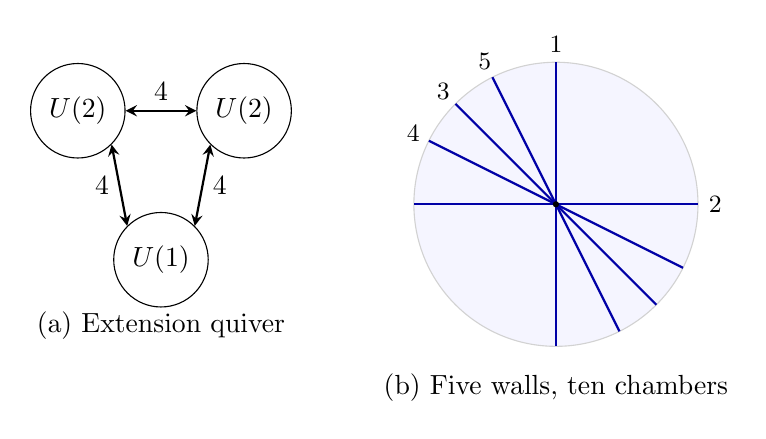
\begin{tikzpicture}[scale=.88,>=stealth]
 \node[circle,draw,minimum size=12mm] (v1) at (-4.7,1.6) {$U(2)$};
 \node[circle,draw,minimum size=12mm] (v2) at (-2.3,1.6) {$U(2)$};
 \node[circle,draw,minimum size=12mm] (v3) at (-3.5,-.55) {$U(1)$};
 \draw[<->,thick] (v1.east)--node[above]{$4$}(v2.west);
 \draw[<->,thick] (v1.south east)--node[left]{$4$}(v3.north west);
 \draw[<->,thick] (v2.south west)--node[right]{$4$}(v3.north east);
 \node at (-3.5,-1.5) {(a) Extension quiver};
 \begin{scope}[xshift=2.2cm,yshift=.25cm]
  \fill[blue!4] (0,0) circle[radius=2.05];
  \draw[gray!35] (0,0) circle[radius=2.05];
  \foreach \ang in {0,90,116.565051,135,153.434949}
    \draw[blue!65!black,thick] (\ang:2.05)--(\ang+180:2.05);
  \fill (0,0) circle[radius=.045];
  \node[font=\small] at (90:2.3) {$1$};
  \node[font=\small] at (0:2.3) {$2$};
  \node[font=\small] at (135:2.3) {$3$};
  \node[font=\small] at (153.434949:2.3) {$4$};
  \node[font=\small] at (116.565051:2.3) {$5$};
  \node at (0,-2.65) {(b) Five walls, ten chambers};
 \end{scope}
\end{tikzpicture}
\end{adjustbox}
\caption{The rank-five example. Each edge in (a) denotes four arrows in
each direction; the diagonal circle acts trivially. In (b) the horizontal
and vertical coordinates are $\zeta_1,\zeta_2$. Wall numbers refer to
Table~\ref{tab:walls}; the bounding circle has no geometric significance.}
\label{fig:quiver-walls}
\end{figure}



For each row take the simple zero-level representations for $d,e$
and scale them into the original bundle chart.
Equivariance preserves their block decomposition.
Theorem~\ref{thm:harmonic-comparison} and the local morphism
identification produce locally free $H$-stable bundles $F_d,F_e$:
their solutions are polystable, and scalar endomorphisms imply
stability. They have
\[
 v_d=\sum_i d_iv(L_i),\qquad v_e=\sum_i e_iv(L_i),\qquad
 \chi(F_d)=\chi(F_e)=0.
\]
Their $H$-slopes vanish, so their reduced $H$-Hilbert polynomials
are equal. Their distinct Mukai vectors make them nonisomorphic.

Along the corresponding line $d\cdot\zeta=0$ their slopes remain
equal. The fixed simple-orbit corrections above balance each
factor at all sufficiently small levels on this line, in the
same holomorphic isomorphism classes. Hence these factors are
stable there and their sum is polystable.
This verifies both the $H$ and the recentered real-class hypotheses
of Theorem~\ref{thm:harmonic-comparison} at every selected point.
We do not assert that all factors at every nearby wall point
are $H$-stable.

For dimension vectors $d,e$ the Mukai pairing is
\begin{equation}\label{eq:triangle-pairing}
 (v_d,v_e)=-2\sum_i d_ie_i
       +4\sum_{i<j}(d_ie_j+d_je_i).
\end{equation}
At these distinct equal-slope stable bundles, Hom in either
direction vanishes; Serre duality and Riemann--Roch identify
\eqref{eq:triangle-pairing} with the cross-extension dimension $k$.
Their self-extension dimensions are $v_d^2+2,v_e^2+2$.
This gives Table~\ref{tab:walls}, with
$\dim U=50-2k$ and transverse dimension $2(k-1)$, summing to $48$.

\subsection{Transverse contractions and metric profiles}
At a fixed selected wall point, the full local representation is
\[
 U\oplus\CC^k\oplus(\CC^k)^*,
\]
with an effective circle trivial on $U$ and of opposite weights
on the two remaining factors. Write them as $(A,B)$.
The equations and complex action are
\[
 BA=0,\qquad \|A\|^2-\|B\|^2=\kappa,\qquad
 z\cdot(A,B)=(zA,z^{-1}B).
\]
At $\kappa>0$, $A\ne0$ determines a line, and $BA=0$ identifies
the quotient with $T^*\PP^{k-1}$.
The negative sign gives the dual projective description.
At zero the invariant $N=AB$ satisfies
$N^2=0$, $\rank N\le1$, and gives the corresponding affine cone.
The two incidence maps are projective, isomorphisms over
$N\ne0$, with zero fiber $\PP^{k-1}$.

These finite contractions transport to actual local analytic
contractions on saturated neighborhoods. The full central analytic
germ is supplied by Theorem~\ref{thm:harmonic-comparison}; the
generic source charts are smooth and holomorphically identified.
For a fixed small $\kappa$, the compact exceptional fiber scales
into radius $R/2$ of a common chart. Properness of the finite
contraction makes the image of its closed complement $\{r\ge R\}$
closed and disjoint from the target origin.
Remove this image and shrink inside the central target chart.
The resulting neighborhood $U_\kappa$ has its entire inverse image
in the source chart. The contraction is therefore defined on a
full saturated neighborhood and remains proper and projective
after analytic transport. Its target neighborhood may depend on
$\kappa$; no uniform saturated radius is required.

\begin{theorem}\label{thm:k3-application}
The rank-five K3 family constructed above has the following
properties for its actual harmonic $L^2$ metric.
\begin{enumerate}
\item Near the three-factor point its full local moduli metrics
have relative error $O(|t|+|u|+r)$ from the doubled-triangle
quotients, uniformly through all stabilizer changes.
Every convergent rescaled parameter direction gives the complete
quotient limit of Theorem~\ref{thm:actual-limits}, including the
five singular wall directions and their intersection.
The finite iterated moving-center limits of
Corollary~\ref{cor:iterated-limits} apply.
\item Each wall in \eqref{eq:five-walls} has selected actual
two-factor strata with the dimensions in Table~\ref{tab:walls}.
Fix such a point and let $\kappa\to0$ with constant sign $\epsilon$.
For any sequence of base points whose balanced representatives divided
by $\sqrt{|\kappa|}$ converge to $(v_*,[A_*,B_*])$, the actual
distances divided by $\sqrt{|\kappa|}$ converge in the pointed
Gromov--Hausdorff sense to the complete product
$U\times T^*\PP^{k-1}$, based at that limit. The transverse factor
carries its flat quotient metric at level $\epsilon\in\{1,-1\}$;
for negative level the projective space has the dual description.
The actual projective exceptional fiber
has the precise $\sqrt{|\kappa|}$ diameter profile
\eqref{eq:fixed-core-scale}.
\item At zero transverse parameter, let $s$ be the nonzero singular
value of $N=AB$ and let $\mathcal S$ denote the local two-factor
stratum. In its recentered coordinates,
\[
 d^{L^2}(f_0(v,N),\mathcal S)
   =(1+O(r))\sqrt{2s}.
\]
At $N=0$ both sides vanish.
\item On the free surrounding zero-level locus,
Proposition~\ref{prop:outer-matching} gives relative matching
error $O(|t|+|u|+r+\|\zeta\|/\lambda)$ whenever
$\|\zeta\|/\lambda\to0$.
\end{enumerate}
\end{theorem}
\begin{proof}
All geometric hypotheses of Theorem~\ref{thm:harmonic-comparison}
and the existence of a module-simple point in the complex zero fiber
are verified above.
Apply Theorems~\ref{thm:actual-limits} and
\ref{thm:moving-centers} for the first assertion.
At a fixed selected wall point, the exact product normal
description and $\sqrt{|\kappa|}$ homogeneity give the second
assertion, including coverage of the whole complete product.
The saturated-domain construction identifies its compact
projective core with the actual contracted fiber.

At zero transverse level, balance gives $\|A\|=\|B\|$.
The unique nonzero singular value of $AB$ is
$s=\|A\|\|B\|$, so transverse distance to the cone vertex is
$\sqrt{\|A\|^2+\|B\|^2}=\sqrt{2s}$.
The Euclidean $U$ factor can be held fixed and cannot reduce
this transverse distance. The two-factor stratum corresponds
exactly to $U\times\{0\}$: its nearby summands stay stable and
nonisomorphic and equivariance preserves their decomposition.
Proposition~\ref{prop:stratum-distance} gives the third assertion,
even when the transverse distance is much smaller than $r$.
The fourth is the previously proved outer matching theorem.
\end{proof}

A vertex-scalar unitary negating every arrow of a triangle would
have scalar ratios $-1$ on each edge, whose product would give
$1=-1$. Thus the sufficient parity hypothesis does not apply here.
We claim the proved linear spatial error, without ruling out
additional cancellations under other normalizations.

The explicit matrices, lattice embedding and pairing formulas
above make the finite data reproducible. An accompanying exact
rational calculation checks all eleven simple representations,
their real and complex moment equations, centralizer dimensions,
and the five wall normals.\footnote{The source and exact calculation
accompany the paper in the
\href{https://github.com/bwuebben/stability-degeneration/tree/main/papers/14_quiver_metric_wall_crossing}{public repository}.}
The analytic conclusions use the
proofs above, not numerical asymptotics. All contractions and
metric limits in this application are local bundle-moduli
statements; no global Gieseker wall-crossing identification or
bubbling compactification is inferred.

